\documentclass[a4paper,11pt]{article}
\usepackage[utf8]{inputenc}
\usepackage[T1]{fontenc}
\usepackage[french]{babel}
\usepackage{makeidx}
\usepackage{textcomp}
\usepackage{graphicx}
\usepackage{mathtools,amssymb,amsthm}
\usepackage{lmodern}
\usepackage{multirow}
\usepackage{array}
\usepackage{longtable}

\title{TER 2019 - Spécifications}
\author{Maxime Gonthier - Benjamin Guillot - Laureline Martin}
\begin{document}
	\pagenumbering{gobble}\clearpage
	\maketitle

\newpage
\tableofcontents

\newpage
\section{Les données}
	On va répartir les données concernant la fac en 4 modules.\\
	\begin{itemize}
		\item Module cours
		\item Module salle de classe
		\item Module étudiant
		\item Module professeur
	\end{itemize}
	\subsection{Module Cours}
		Le module cours est une classe représentant un cours sur un temps donné.\\
		Lors des affectations, on modifiera pour chaque instance a deplacer l'horaire de début.\\
		Elle contient : 
		\begin{enumerate}
			\item Durée : un entier -représente la durée du cours en minutes-
			\item Une liste des étudiants : un tableau d'entier qui contient les numero des étudiants participant à ce cours.
			\item Le type de salle utilisé : un entier, 0 pour une salle de TP et 1 pour un autre salle (on pourra ajouter d'autres type de salle si necessaire).
			\item Un indice de flexibilité calculé en fonction de celle des etudiants : somme des flexibilité de chaque étudiants (cette modelisation a pour but de favoriser les cours ayant le plus d'etudiants).
			\item Le nombres d'étudiant : un entier
			\item Un numéro de salle : un entier (identifiant unique représentant la salle)
			\item Le numéro du professeur donnant ce cours : un entier (identifiant unique représentant le professeur)
			\item L'horaire de début : un entier pour l'heure, un entier pour la minute (structure implémentée specialement pour le projet)  
			\item L'horaire de fin : un entier pour l'heure, un entier pour la minute.
		\end{enumerate}
	\subsection{Module Salle de classe}
		Le module salle représente la localisation du cours sur un temps donné.
		\begin{enumerate}
			\item Numéro de salle : un entier (identifiant unique)
			\item Une localisation : un entier -0 pour proche de l'arrêt, 1 pour modérément éloigné, 2 pour éloigné-. 
			\item Un type de salle : un entier, 0 pour une salle de TP et 1 pour une autre salle (on pourra ajouter d'autres type de salle si necessaire).
			\item Une capacité maximale : un entier
		\end{enumerate}
	\subsection{Module Etudiant}
		Le module étudiant représente un élève sur le temps d'exécution du programme.
		\begin{enumerate}
			\item Distance entre son domicile et l'université : un entier, 0 si l'étudiant habite a moins de 15 min de la fac, 1 si il habite entre 15 et 45 min de la fac, 2 sinon.
			\item Flexibilité : un entier calculé en fonction de la distance de trajet et des contraintes forte et faible. 
			\end{enumerate}
	\subsection{Module Professeur}
		Le module professeur représente un professeur sur le temps d'exécution du programme.
		\begin{enumerate}
			\item Un numéro de professeur : un entier (identifiant unique)
			\item plage de disponibilité début : un entier pour l'heure, un entier pour la minute.
			\item plage de disponibilité fin : un entier pour l'heure, un entier pour la minute.
			\end{enumerate}
	\subsection{Conclusion des liens entre les modules}
		\centerline{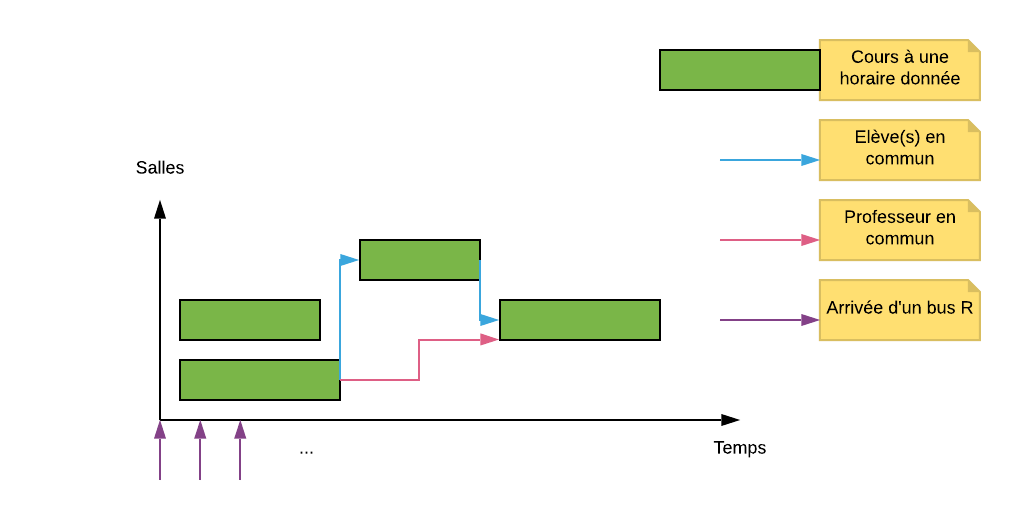
\includegraphics[scale=0.5]{modelter.png}}
		Modélisation.\\

\section{Contraintes}
	Pour optimiser, nous faisons face à plusieurs contraintes, toutes ne sont pas 
	de même "importances". Nous allons donc devoir définir un ordre de priorité sur 
	les contraintes, ainsi lors de l'optimisation par notre algorithme, nous 
	pourrons ajuster et obtenir de meilleurs résultats même si certaines contraintes
	"faibles" sont violées.\\
	\subsection{Contraintes dures}
		\begin{enumerate}
			\item 0 : Salle utilisée par deux cours différents pour des horaires 
			qui se chevauchent
			\item 1 : Un élève qui suit deux cours dont les horaires se chevauchent
			\item 2 : Avoir une personne à charge ce qui impose un horaire le matin et/ou le soir.
			Exemple : Sois X l'heure de début d'un cours, si un enfant doit être déposé à l'école à 9h on a : X > 9 + (indice de distance de cet étudiant)*30 min
			Sois Y l'heure de fin d'un cours, si un enfant doit être récupéré à l'école à 17h on a : Y < 17 - (indice de distance de cet étudiant)*30 min			
		\end{enumerate}
	\subsection{Contraintes faibles}
		\begin{enumerate}
			\item 3 : Avoir un travail, cela impose la même chose que la contraintes précédentes
		\end{enumerate}

	\subsection{Module Contraintes}  
		\begin{itemize}
			\item identifiant : un entier non unique correspondant à une des contrainte precedement. L'identifiant représente une hierarchie dans les contraintes, de la plus forte a la plus faible 
			\item un tableau d'entier contenant les identifiant des étudiants sujet à cette contrainte.
	%\subsection{Sélections par heuristiques}
		%Les différentes heuristiques que nous allons utiliser pour jouer sur les 
		%contraintes. $$surement tabou$$ \\
		\end{itemize}
\section{Affectation}
	On va affecter chaque cours à un horaires sans prendre en compte les transports. On ne va utiliser que les contraintes énoncés précédemment. \\
	On va utiliser une heuristique tabou. On commence avec un emploi du temps par défaut. Le voisinage correspond à la modification d'un cours. A chaque itération on recalcule le nombre de contraintes violées. Un optimum local sera une solution viable, c'est à dire qui ne viole pas les deux contraintes les plus fortes. 
	
\section{Evaluation de chaque affectation}
	On évalue ensuite chaque optimum local trouvé afin de définir lequel viole le moins de contraintes. Elle correspond à la somme des contraintes violées. Les contraintes sont hiérarchisées comme vu précédemment, ainsi lors de la somme des contraintes on pondère en fonction de cette hiérarchisation.
	
\section{Début de reflexion sur l'implémentation des transports}
	Pour les transports, on supposera que chaque élève arrivera par le bus précédant le début du premier cours de sa journée. De cette manière a chaque itération de l'affectation des cours, on pourra recalculer la congestion de chaque bus (qui sera utilisé comme fonction objectif du projet une fois les transport implémentés).La congestion peut être représentée par le pourcentage de remplissage du bus à chaque arrêt. 

\end{document}
